\section{Introduction}
\label{sec-intro}

Graph analytics systems must handle very large graphs such as the Facebook friends graph with more than a billion nodes and 200 billion edges, or the indexable Web graph, which has around 100 billion nodes and trillions of edges. We need parallel computing to process graphs of this size with reasonable performance. GPUs are a popular platform for improving the performance of graph analytical systems, due to their high parallelism. However, these large graphs containing billions of nodes and trillions of edges cannot be processed using the capacity of the memory of a single GPU. 

One common solution to process the large graphs is to partition the large graphs across a cluster of machines and GPUs. The graphs are partitioned between the machines, and the communication is handled using a substrate like MPI. The best-performing graph partitioning strategy depends on the algorithm, input graph and number of hosts. While the partitioning of graphs to a cluster of machines makes sure that the GPUs work in parallel and make the computations fast, the performance is bottlenecked by the communication overhead between the different partitions. Also, since different graphs and algorithms need different partitioning policies, a key challenge in distributed graph analytics frameworks is to optimize the communication while supporting heterogeneous partitioning policies. 

\begin{figure}
\centering
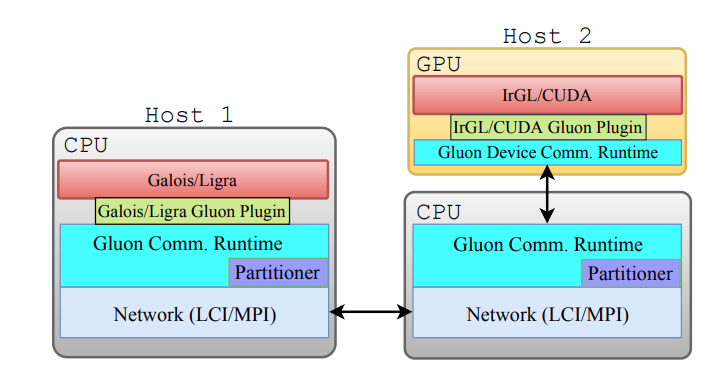
\includegraphics[width=0.49\textwidth]{gluon.png}
\mycaption{Gluon Overview}{The figure provides an overview of the Gluon Communication Substrate. 
}
\label{fig-gluon}
%\vspace{-20pt}
\end{figure}

D-IrGL is a distributed multi-GPU graph analytical framework. It supports multi-host multi-GPU architectures. D-IrGL uses the IrGL compiler for performing computations on each partition independently, and then uses the Gluon communication substrate for communicating and synchronizing data between the different GPUs. The performance of D-IrGL for different graphs depends mainly on the performance of the Gluon communication substrate. Figure~\ref{fig-gluon} shows the basic overview of the Gluon communication substrate. 

The limitation in the current Gluon implementation is that it does not use the features that are available in modern GPU architectures such as asynchronous data transfers, unified memory, or direct GPU-GPU communication without the involvement of CPUs. Since these features are independent of the graphs themselves, accommodating these features inside Gluon will improve the performance of all the graphs that use Gluon for communication. In this project, we  investigate the different features that have been added to the recent NVIDIA GPUs, and we attempt to apply them to the Gluon substrate and evaluate the performance of a simple BFS push algorithm for large graphs. 

The contributions that we make in this project are as follows:
\begin{enumerate}
\item We use streaming transfers of data between GPU and CPU of a node to overlap computation of data at the GPU along with communication of data between different nodes via CPU. 
\item We use Unified Virtual Addressing (UVA) to store the data of the graphs, to store larger partitions on each node. 
\item We attempt to implement inter-GPU communication of graph data without the involvement of CPU, among the GPUs located in a single machine as well as GPUs located across multiple machines. 
\end{enumerate}
